\documentclass[11pt]{article}

\usepackage[a4paper,margin=1in]{geometry}
\usepackage{amsmath}
\usepackage{amssymb}
\usepackage{booktabs}
\usepackage{tabularx}
\usepackage{graphicx}
\usepackage[hidelinks]{hyperref}
\usepackage[authoryear,round]{natbib}
\usepackage{siunitx}
\usepackage{tikz}
\usetikzlibrary{arrows.meta,positioning}
\sisetup{group-separator={,}, group-minimum-digits=4}

\graphicspath{%
  {../../design_dataset/report/outputs/figures/}%
  {../../class_imbalance/outputs/figures/}%
}

\title{Computational Pathology and Benchmark Datasets:\\
An Introduction to the Domain and Data}
\author{Yannik Queisler}
\date{\today}

\begin{document}
\maketitle

\begin{abstract}
\noindent This report introduces the domain of computational pathology and the public datasets used
in this thesis. It first explains what diagnostic pathology is, how a stained glass slide becomes a
gigapixel whole-slide image, why such images are tiled into patches, and how weakly supervised and
frozen foundation-model pipelines turn those patches into predictions. It then describes, in detail,
four H\&E datasets --- CAMELYON16, TCGA-UT, BRACS, and PANDA --- presented in the order of the
diagnostic question they pose, from detection (\emph{is cancer present?}) through cancer typing and
lesion subtyping to ordinal grading (\emph{how aggressive is it?}). Each dataset is given with its
clinical background, an example patch, a summary table, and its class distribution.
\end{abstract}

\setcounter{tocdepth}{2}
\tableofcontents
\clearpage

\section{Computational Pathology}
\label{sec:cpath}
Diagnostic pathology is the branch of medicine that examines tissue under the microscope to detect
and characterise disease. When cancer is suspected, a biopsy or surgical resection is fixed, thinly
sectioned, mounted on a glass slide, and stained --- most commonly with hematoxylin and eosin
(H\&E), which colours cell nuclei blue-purple and cytoplasm and stroma shades of pink --- so that a
pathologist can read cellular and tissue morphology and render a diagnosis. This reading is the
clinical reference standard for cancer detection, typing, and grading, and it drives treatment
decisions. It is also labour-intensive, requires scarce expertise, and is subject to inter- and
intra-observer variability, which motivates computational assistance
\citep{madabhushi2016imageAnalysis,song2023aiPathology}.

Computerised analysis of microscopy images is not new: the earliest work on cell and chromosome
image analysis dates back more than fifty years \citep{madabhushi2016imageAnalysis}. What changed
recently is scale and method. \emph{Digital pathology} digitises the glass slide with a
whole-slide scanner, enabling telepathology, archiving, and education; \emph{computational
pathology} (CPath) goes further, treating the resulting images as high-dimensional data for
quantitative, reproducible analysis and integrating them with clinical and molecular context
\citep{abels2019computationalPathology,hosseini2024computationalPathology}. A useful distinction
here is between the \emph{ground truth}, the abstract label one wishes to predict, and the
\emph{gold standard}, the practical benchmark used to approximate it --- typically a pathologist's
own assessment. Because algorithmic outputs can eventually prove more reproducible than the human
benchmark that trained them, CPath must navigate a \emph{gold-standard paradox} in which the
reference itself is imperfect \citep{abels2019computationalPathology}.

The clinical value of CPath is usually framed along two axes \citep{song2023aiPathology,madabhushi2016imageAnalysis}.
\emph{Automation} standardises tasks pathologists already perform --- detecting metastases,
subtyping and grading tumours, quantifying immunohistochemical markers --- reducing workload and
observer variability. \emph{Discovery} identifies signatures beyond human visual limits, such as
predicting prognosis, therapy response, or molecular alterations (for example microsatellite
instability) directly from H\&E morphology; these are the ``sub-visual'' features that quantitative
analysis can mine but a human eye cannot reliably see \citep{madabhushi2016imageAnalysis}.
Table~\ref{tab:cpath-tasks} summarises representative tasks. The datasets in this report all sit
on the automation axis: each carries a diagnostic label a pathologist established, and the task is
to predict it from H\&E tissue.

\begin{table}[ht]
  \centering
  \small
  \begin{tabularx}{\linewidth}{@{}lX@{}}
    \toprule
    Role & Representative tasks\\
    \midrule
    Automation & Metastasis detection; cancer-type classification; tumour subtyping; Gleason/ISUP
                 grading; mitosis counting; immunohistochemistry (PD-L1, Ki-67) quantification\\
    Discovery  & Prognosis and recurrence-risk prediction; molecular-marker prediction (e.g.\
                 microsatellite instability) from H\&E; therapy-response biomarkers\\
    \bottomrule
  \end{tabularx}
  \caption{Two roles of computational pathology, following \citet{song2023aiPathology} and
  \citet{madabhushi2016imageAnalysis}. The datasets in this report are automation tasks with
  pathologist-established labels.}
  \label{tab:cpath-tasks}
\end{table}

\subsection{The whole-slide imaging pipeline}
\label{sec:pipeline}
A digitised slide is a \emph{whole-slide image} (WSI): a single H\&E image of an entire tissue
section, routinely on the order of \num{100000}$\times$\num{100000} pixels and \num{0.5}--\num{4}\,GB
in size \citep{song2023aiPathology,abels2019computationalPathology}. To make this tractable, a WSI is
stored as a \emph{pyramid} of progressively downsampled copies, so the same slide can be read at
several magnifications (Table~\ref{tab:magnification}): high magnification resolves nuclear detail
and mitoses, while lower magnifications carry the tissue-architectural context that diagnosis also
depends on. Scanning the whole section, rather than a manually chosen field of view, removes
selection bias and captures intratumoral heterogeneity, but it produces far more data than fits in
GPU memory.

\begin{table}[ht]
  \centering
  \small
  \begin{tabularx}{\linewidth}{@{}llX@{}}
    \toprule
    Magnification & Resolution & What it resolves\\
    \midrule
    \num{40}$\times$ & ${\approx}\num{0.25}\,\mu$m/pixel & Nuclear detail, chromatin, mitotic figures\\
    \num{20}$\times$ & ${\approx}\num{0.5}\,\mu$m/pixel  & Cellular morphology, individual glands\\
    \num{10}$\times$ & ${\approx}\num{1.0}\,\mu$m/pixel  & Local tissue architecture\\
    \num{5}$\times$  & ${\approx}\num{2.0}\,\mu$m/pixel  & Macro-architectural context\\
    \bottomrule
  \end{tabularx}
  \caption{Typical magnification levels of a pyramidal WSI and the morphology each makes legible
  \citep{song2023aiPathology}. High magnifications are needed for nuclear grading, lower ones for
  architectural context.}
  \label{tab:magnification}
\end{table}

The standard response to the size of a WSI is a divide-and-conquer strategy: the image is
partitioned into small \emph{patches} (also called \emph{tiles}), for example $256\times256$ pixels,
each processed independently and later aggregated into a slide- or patient-level prediction
\citep{song2023aiPathology}. Figure~\ref{fig:pipeline} sketches the resulting pipeline, from stained
slide to prediction, that every dataset in this report passes through.

\begin{figure}[ht]
  \centering
  \resizebox{\textwidth}{!}{%
  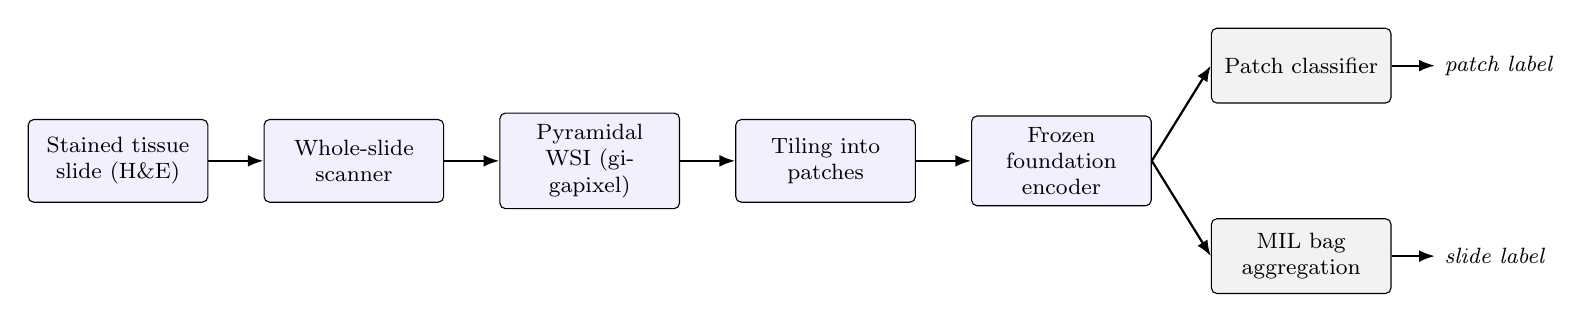
\begin{tikzpicture}[
    node distance=0.55cm and 0.7cm,
    stage/.style={draw, rounded corners=2pt, align=center, fill=blue!6, inner sep=4pt,
                  font=\footnotesize, text width=2.0cm, minimum height=1.05cm},
    head/.style={draw, rounded corners=2pt, align=center, fill=gray!10, inner sep=4pt,
                 font=\footnotesize, text width=2.0cm, minimum height=0.95cm},
    lab/.style={font=\footnotesize\itshape},
    arrow/.style={-{Latex[length=2mm]}, thick}
  ]
    \node[stage] (slide) {Stained tissue slide (H\&E)};
    \node[stage, right=of slide] (scan) {Whole-slide scanner};
    \node[stage, right=of scan] (wsi) {Pyramidal WSI (gigapixel)};
    \node[stage, right=of wsi] (patch) {Tiling into patches};
    \node[stage, right=of patch] (enc) {Frozen foundation encoder};
    \node[head, above right=0.15cm and 0.75cm of enc] (phead) {Patch classifier};
    \node[head, below right=0.15cm and 0.75cm of enc] (mhead) {MIL bag aggregation};
    \node[lab, right=0.55cm of phead] (plabel) {patch label};
    \node[lab, right=0.55cm of mhead] (slabel) {slide label};
    \draw[arrow] (slide)--(scan);
    \draw[arrow] (scan)--(wsi);
    \draw[arrow] (wsi)--(patch);
    \draw[arrow] (patch)--(enc);
    \draw[arrow] (enc.east) -- (phead.west);
    \draw[arrow] (enc.east) -- (mhead.west);
    \draw[arrow] (phead)--(plabel);
    \draw[arrow] (mhead)--(slabel);
  \end{tikzpicture}%
  }
  \caption{The computational-pathology pipeline used throughout the benchmarks. A stained slide is
  scanned into a pyramidal WSI and tiled into patches; a frozen foundation-model encoder embeds each
  patch once, after which either a patch classifier predicts a per-tile label or a multiple-instance
  head aggregates the patch features of a slide into a slide-level prediction.}
  \label{fig:pipeline}
\end{figure}

\subsection{Learning from patches: weak supervision and foundation models}
\label{sec:learning}
How labels attach to these units determines the learning regime. When each patch carries a reliable
label --- because it was cropped from a pathologist-selected region, or intersected with an expert
pixel mask --- ordinary patch classification applies. When only a slide-level diagnosis is
available, the problem is \emph{weakly supervised}: the slide is a \emph{bag} of patch
\emph{instances} that share one label, and \emph{multiple-instance learning} (MIL) aggregates the
instances --- typically through a learned attention mechanism that weights diagnostically salient
patches --- into a slide prediction \citep{song2023aiPathology,hosseini2024computationalPathology}.
Because tiling discards spatial context, context-aware models such as graph neural networks (over
patches or nuclei) and transformers (with global self-attention) are sometimes used to recover it,
but the attention-MIL bag remains the workhorse for slide-level tasks. Both regimes appear in the
datasets below, and two of them (CAMELYON16 and PANDA) support both on the same slides.

The features fed to these heads have shifted from hand-crafted descriptors --- interpretable
measurements of nuclear shape, texture, or spatial architecture --- to learned representations that
capture patterns beyond human perception \citep{madabhushi2016imageAnalysis}. Modern CPath rarely
trains an image encoder from scratch: a pathology \emph{foundation model}, pre-trained
self-supervised on large slide archives, provides a frozen feature extractor that embeds each patch
once into a fixed-length vector, leaving only a lightweight classifier or MIL head to train. The
benchmarks that build on this report use Virchow2, one such H\&E foundation model, as a frozen
encoder \citep{vorontsov2024virchow,zimmermann2024virchow2}. Freezing the representation isolates the
effect being studied --- here, class imbalance --- from the confounds of end-to-end backbone
training, and makes the patch and MIL regimes directly comparable, because both consume the same
embeddings.

\subsection{Data, annotation, and the challenge of class imbalance}
\label{sec:data-challenge}
Deep learning is data-hungry, and expert annotation is the binding constraint in CPath: pathologist
labelling is slow, expensive, and hard to scale, so datasets range from densely mask-annotated
cohorts to those carrying only a single slide-level diagnosis
\citep{abels2019computationalPathology,hosseini2024computationalPathology}. The four datasets in
this report deliberately span that range of annotation form. A second, pervasive property of
clinical tissue cohorts is that they are \emph{imbalanced}. Common tumour types and benign tissue
dominate, while the categories that matter most for a patient --- rare cancers, precancerous
atypia, small metastatic foci --- are scarce. A model can post a high overall accuracy while failing
exactly on these under-represented classes, so imbalance is a concern for both training and
evaluation. The next section introduces the datasets, together with a simple measure that makes the
imbalance of a class distribution quantitative and comparable across datasets.

\section{Datasets}
\label{sec:datasets}
Four public H\&E datasets are used, described here in the order of the diagnostic question they
pose --- an arc that also escalates the structure of the label and varies the organ and the form of
annotation:

\begin{itemize}
  \item \textbf{CAMELYON16} --- \emph{is cancer present?} Binary metastasis \emph{detection} in
        sentinel lymph nodes, with pixel-mask annotations.
  \item \textbf{TCGA-UT} --- \emph{what cancer is it?} Pan-cancer \emph{typing} across 32 organs,
        each patch labelled with its slide's cancer type.
  \item \textbf{BRACS} --- \emph{how abnormal is this tissue?} Breast-lesion \emph{subtyping} along
        the benign--atypical--malignant continuum, with region-of-interest annotations.
  \item \textbf{PANDA} --- \emph{how aggressive is it?} Ordinal ISUP \emph{grading} of prostate
        biopsies, with region masks and built-in two-provider heterogeneity.
\end{itemize}

\paragraph{Measuring class imbalance.}
Two numbers summarise how skewed a dataset's class distribution is. The head-to-tail ratio --- the
largest class support divided by the smallest --- is intuitive, but it reads only the two extreme
classes and ignores the number of classes $K$, so it cannot fairly compare a two-class cohort with a
thirty-two-class one. An entropy-based measure complements it. For empirical class proportions
$p_1,\dots,p_K$ (with $\sum_i p_i=1$), let the Shannon entropy be $H(p)=-\sum_{i=1}^{K} p_i \log p_i$,
whose maximum, attained by the uniform distribution, is $\log K$. Normalising and complementing gives
\begin{equation}
  \label{eq:imbalance}
  \text{imbalance} \;=\; 1 - H_{\mathrm{norm}} \;=\; 1 - \frac{-\sum_{i=1}^{K} p_i \log p_i}{\log K}
  \;\in\; [0,1],
\end{equation}
where \num{0} is a perfectly balanced distribution and values closer to \num{1} indicate stronger
imbalance. Because the $\log K$ normalisation removes the dependence on the number of classes, this
measure is comparable across datasets, unlike the raw ratio. It is reported in each dataset's summary
table at both \emph{tile} and \emph{slide} level, since the two can differ substantially when tile
labels are derived from masks rather than inherited from the slide.

\subsection{CAMELYON16 --- lymph-node metastasis detection}
\label{sec:camelyon16}
CAMELYON16 is an organ-specific H\&E cohort of sentinel lymph-node sections for the detection of
breast-cancer metastases \citep{bejnordi2017diagnostic,litjens2018gigascience}. The diagnostic
question is the most basic in oncology --- \emph{is cancer present?} --- and the label is binary:
each slide is either \emph{normal} or contains \emph{tumor} (metastasis). Expert annotations are
supplied as pixel-level masks marking tumour tissue, rather than as cropped regions, so individual
tiles can be labelled by intersecting them with the mask.

The benchmark uses \num{398} of the \num{399} published slides (\num{160} tumor, \num{238} normal)
after excluding one slide without usable tile evidence; each slide is its own patient, so
slide-disjoint splits coincide with patient-disjoint splits. Because metastatic tissue occupies only
a small fraction of a sectioned node, mask-derived tumor tiles are scarce: the patch distribution is
\num{2340040} normal against \num{59672} tumor tiles, a head-to-tail ratio of
approximately $\num{39}{:}1$ and an entropy-based imbalance of $1-H_{\mathrm{norm}}\approx\num{0.83}$
--- the most severe in the suite despite being the simplest task (Table~\ref{tab:camelyon16-summary},
Figure~\ref{fig:camelyon16-dist}). At the slide level, however, tumour and normal slides are almost
balanced (\num{160} versus \num{238}; $1-H_{\mathrm{norm}}\approx\num{0.03}$): the severe imbalance is
a within-slide effect, since tumour tiles are scarce even on slides that do contain a metastasis. The
\num{20} tumor slides whose annotations are not exhaustive are excluded from the tile-labelling
regime, where unannotated tumour could be mislabelled as normal, but retained where only the reliable
slide-level label is used.

\begin{table}[ht]
  \centering
  \begin{minipage}{0.32\linewidth}
    \centering
    \IfFileExists{../../design_dataset/report/outputs/figures/camelyon16_example_patch.jpg}{%
      
\includegraphics[width=\linewidth]{camelyon16_example_patch.jpg}%
    }{%
      \fbox{\parbox{0.85\linewidth}{\centering\vspace{2em}CAMELYON16 example tile unavailable.\vspace{2em}}}%
    }
  \end{minipage}
  \hfill
  \begin{minipage}{0.62\linewidth}
    \centering
    \small
    \begin{tabular}{ll}
      \toprule
      Property & Value\\
      \midrule
      WSIs (tumor / normal) & \num{160} / \num{238}\\
      Patch-labelled WSIs & \num{378}\\
      WSI-bag size (median tiles) & \num{7874}\\
      Tile labels & tumor, normal\\
      Tumor / normal tiles & \num{59672} / \num{2340040}\\
      Imbalance $1-H_{\mathrm{norm}}$ (tile) & \num{0.832}\\
      Imbalance $1-H_{\mathrm{norm}}$ (slide) & \num{0.028}\\
      \bottomrule
    \end{tabular}%
  \end{minipage}
  \caption{CAMELYON16 dataset properties, alongside an example $256\times256$ tumor tile. The
  WSI-bag size is the data-driven median of available tissue tiles per slide. Imbalance is far more
  severe at tile than at slide level, because tumour tiles are rare even within tumour slides.}
  \label{tab:camelyon16-summary}
\end{table}

\begin{figure}[ht]
  \centering
  \IfFileExists{../../design_dataset/report/outputs/figures/camelyon16_class_distribution.png}{%
    
\includegraphics[width=0.6\linewidth]{camelyon16_class_distribution.png}%
  }{%
    \fbox{\parbox{0.7\linewidth}{\centering CAMELYON16 patch distribution figure unavailable.}}%
  }
  \caption{CAMELYON16 patch support by tumor/normal label after mask-based labelling
  (log scale). Tumor tiles are roughly \num{39} times scarcer than normal tiles.}
  \label{fig:camelyon16-dist}
\end{figure}

\subsection{TCGA-UT --- pan-cancer typing}
\label{sec:tcgaut}
TCGA-UT widens the lens from one organ to the whole body. It is derived from diagnostic WSIs in The
Cancer Genome Atlas (TCGA), a pan-cancer resource linking molecular and clinical data with large
image collections \citep{tomczak2015reviewThe}. The TCGA-UT release turns this slide archive into a
computational-pathology dataset by cropping H\&E tumour patches from pathologist-selected uniform
tumour regions: \num{1608060} RGB patches of $256\times256$ pixels from \num{8736} diagnostic slides,
across \num{32} cancer types \citep{komura2022universalEncoding}. Every patch carries the cancer-type
label of the slide it was cropped from, so the patches are themselves labelled samples --- the unit
of patch-level classification --- while their slide identities also allow grouping into slide-level
bags. The labels are cancer types, not dense pixel masks or cell-level annotations, so the diagnostic
question is \emph{what cancer is it?}, a nominal classification across 32 organs.

The largest class is glioblastoma multiforme (GBM; \num{792} slides) and the smallest is diffuse
large B-cell lymphoma (DLBC; \num{28} slides), a slide-level head-to-tail ratio of \num{28.3}. Yet
spread across 32 gradually declining classes this is only a mild entropy-based imbalance
($1-H_{\mathrm{norm}}\approx\num{0.09}$; Table~\ref{tab:tcgaut-summary}, Figure~\ref{fig:tcgaut-dist})
--- a first illustration that the head-to-tail ratio and the $K$-aware measure need not agree.

\begin{table}[ht]
  \centering
  \begin{minipage}{0.30\linewidth}
    \centering
    \IfFileExists{../../class_imbalance/outputs/figures/tcga_ut_example_patch.jpg}{%
      
\includegraphics[width=\linewidth]{tcga_ut_example_patch.jpg}%
    }{%
      \fbox{\parbox{0.85\linewidth}{\centering\vspace{2em}TCGA-UT example patch unavailable.\vspace{2em}}}%
    }
  \end{minipage}
  \hfill
  \begin{minipage}{0.64\linewidth}
    \centering
    \small
    \begin{tabular}{ll}
      \toprule
      Property & Value\\
      \midrule
      Cancer-type labels & \num{32}\\
      Diagnostic slides & \num{8736}\\
      Patches & \num{1608060} of $256\times256$\\
      Largest class & Glioblastoma (GBM), \num{792} slides\\
      Smallest class & B-cell lymphoma (DLBC), \num{28} slides\\
      Imbalance $1-H_{\mathrm{norm}}$ (patch) & \num{0.085}\\
      Imbalance $1-H_{\mathrm{norm}}$ (slide) & \num{0.085}\\
      \bottomrule
    \end{tabular}
  \end{minipage}
  \caption{TCGA-UT dataset properties, alongside an example $256\times256$ H\&E tumor patch. Because
  every patch inherits its slide's label, the tile- and slide-level imbalance coincide.}
  \label{tab:tcgaut-summary}
\end{table}

\begin{figure}[ht]
  \centering
  \IfFileExists{../../class_imbalance/outputs/figures/class_distribution.png}{%
    
\includegraphics[width=0.86\linewidth]{class_distribution.png}%
  }{%
    \fbox{\parbox{0.7\linewidth}{\centering TCGA-UT cancer-type distribution figure unavailable.}}%
  }
  \caption{TCGA-UT slide support by cancer-type rank. The imbalance is moderate once spread
  over \num{32} classes, with a head-to-tail ratio of \num{28.3}.}
  \label{fig:tcgaut-dist}
\end{figure}

\subsection{BRACS --- breast-lesion subtyping}
\label{sec:bracs}
BRACS narrows back to a single organ but sharpens the question from \emph{which cancer} to
\emph{how abnormal is this tissue}. It is an H\&E breast-pathology dataset of \num{547} WSIs and
\num{4539} regions of interest (ROIs) from \num{189} patients, annotated by consensus of three
board-certified pathologists \citep{brancati2022bracs}. The labels form three lesion types ---
benign, atypical, and malignant --- refined into seven subtypes: normal (N), pathological benign
(PB), usual ductal hyperplasia (UDH), flat epithelial atypia (FEA), atypical ductal hyperplasia
(ADH), ductal carcinoma in situ (DCIS), and invasive carcinoma (IC). Annotations are ROI crops
rather than whole-slide labels or pixel masks, and a single slide may contain ROIs of several
subtypes.

The benchmark uses the seven-subtype target, the level at which imbalance is most relevant: the
atypical lesions FEA and ADH are clinically important, comparatively scarce precancers that
collapsing to three lesion types would hide. After deterministic ROI tiling into $256\times256$
patches, \num{387} of the \num{547} WSIs contribute at least one annotated tile; the prepared cohort
spans \num{151} patients, the full \num{4539} ROI records, and \num{99352} patches. Counting the
slides that contain each subtype (a slide with several lesions counts under each), support ranges
from PB (\num{196} slides) at the head to DCIS (\num{87} slides) at the tail, a mild head-to-tail
ratio of approximately $\num{2.3}{:}1$ and an entropy-based imbalance of only
$1-H_{\mathrm{norm}}\approx\num{0.02}$ (Table~\ref{tab:bracs-summary},
Figure~\ref{fig:bracs-dist}). BRACS is thus a genuine but mild imbalance setting whose difficulty
comes from fine-grained morphology rather than a steep tail.

\begin{table}[ht]
  \centering
  \begin{minipage}{0.32\linewidth}
    \centering
    \IfFileExists{../../design_dataset/report/outputs/figures/bracs_example_patch.jpg}{%
      
\includegraphics[width=\linewidth]{bracs_example_patch.jpg}%
    }{%
      \fbox{\parbox{0.85\linewidth}{\centering\vspace{2em}BRACS example ROI patch unavailable.\vspace{2em}}}%
    }
  \end{minipage}
  \hfill
  \begin{minipage}{0.62\linewidth}
    \centering
    \small
    \begin{tabular}{ll}
      \toprule
      Property & Value\\
      \midrule
      Patients & \num{151}\\
      WSIs with ROI tiles & \num{387}\\
      ROI tiles & \num{99352}\\
      WSI-bag size (median tiles) & \num{360}\\
      Subtype labels & N, PB, UDH, FEA, ADH, DCIS, IC\\
      Imbalance $1-H_{\mathrm{norm}}$ (tile) & \num{0.072}\\
      Imbalance $1-H_{\mathrm{norm}}$ (slide) & \num{0.018}\\
      \bottomrule
    \end{tabular}%
  \end{minipage}
  \caption{BRACS dataset properties, alongside an example $256\times256$ ROI tile. Slide-level support
  counts each slide under every subtype it contains; the tile-level distribution weights subtypes by
  their tile counts, making it somewhat more skewed.}
  \label{tab:bracs-summary}
\end{table}

\begin{figure}[ht]
  \centering
  \IfFileExists{../../design_dataset/report/outputs/figures/bracs_class_distribution.png}{%
    
\includegraphics[width=0.72\linewidth]{bracs_class_distribution.png}%
  }{%
    \fbox{\parbox{0.7\linewidth}{\centering BRACS subtype distribution figure unavailable.}}%
  }
  \caption{BRACS WSI support by seven-subtype label (slides containing each subtype), from PB
  at the head to DCIS at the tail.}
  \label{fig:bracs-dist}
\end{figure}

\subsection{PANDA --- prostate cancer grading}
\label{sec:panda}
PANDA (Prostate cANcer graDe Assessment) poses the most nuanced question --- \emph{how aggressive is
the cancer?} --- as an ordinal grading problem. It is an H\&E dataset of prostate core-needle biopsies
assembled for automated Gleason grading and the largest public cohort of its kind, with \num{10616}
whole-slide biopsies \citep{bulten2022panda}. Gleason grading describes prostate-cancer severity from
glandular growth patterns; pathologists summarise the dominant and secondary malignant patterns into
ordinal ISUP Grade Groups, where higher groups indicate more aggressive morphology. Here grade
\num{0} marks benign tissue and grades \num{1}--\num{5} are the ordered ISUP cancer groups.

PANDA differs from the other three along every axis a generality check exercises: a third organ
(prostate), an ordinal rather than nominal or binary label, and a built-in source of heterogeneity,
because the slides come from two institutions --- Radboud University Medical Center and Karolinska
Institute --- that differ in staining, scanning, and annotation convention, and grade differently
(Karolinska biopsies concentrate at low grades, Radboud spread more evenly). To keep frozen-feature
extraction tractable on a cohort an order of magnitude larger than the others, the benchmark draws a
stratified subset of approximately \num{2000} biopsies preserving the joint distribution of ISUP grade
and provider. The ISUP distribution is mildly imbalanced, from ISUP\,0 (\num{544} biopsies) to
ISUP\,5 (\num{230}), a ratio of approximately $\num{2.4}{:}1$ and an entropy-based imbalance of
$1-H_{\mathrm{norm}}\approx\num{0.04}$. PANDA's masks additionally support a provider-consistent
binary cancer/benign tile label --- the only labelling the two institutions share --- giving
\num{580531} benign against \num{122751} cancer tiles (approximately $\num{4.7}{:}1$,
$1-H_{\mathrm{norm}}\approx\num{0.33}$), so the same biopsies furnish both an ordinal slide-level
grading target and a binary tile-level detection target (Table~\ref{tab:panda-summary},
Figure~\ref{fig:panda-dist}).

PANDA is the only one of the four datasets whose two regimes answer different questions, and this
follows from its annotations rather than from a design choice. It is the one cohort carrying two
independent label sources at two granularities: a slide-level ordinal ISUP grade, which summarises
the whole biopsy and cannot be assigned to a single tile, and pixel masks that yield a per-tile label.
CAMELYON16, TCGA-UT, and BRACS instead each provide a single label concept --- tumour/normal, cancer
type, or lesion subtype --- that applies unchanged at both tile and slide level, so their two regimes
share one task and differ only in prediction unit.

\begin{table}[ht]
  \centering
  \small
  \begin{tabular}{ll}
    \toprule
    Property & Value\\
    \midrule
    WSIs (biopsies) & \num{2000}\\
    Patch-labelled WSIs & \num{1984}\\
    WSI-bag size (median tiles) & \num{421}\\
    WSI labels / tile labels & ISUP 0--5 / benign, cancer\\
    Benign / cancer tiles & \num{580531} / \num{122751}\\
    Imbalance $1-H_{\mathrm{norm}}$ (tile, cancer/benign) & \num{0.332}\\
    Imbalance $1-H_{\mathrm{norm}}$ (slide, ISUP) & \num{0.043}\\
    \bottomrule
  \end{tabular}
  \caption{PANDA dataset properties after stratified subset selection and mask-based patch labelling.
  The WSI-bag size is the data-driven median of available tissue tiles per biopsy. Unlike the other
  datasets, the tile and slide regimes carry different labels (binary cancer/benign vs six-class
  ISUP), so their imbalance figures describe two different tasks.}
  \label{tab:panda-summary}
\end{table}

\begin{figure}[ht]
  \centering
  \IfFileExists{../../design_dataset/report/outputs/figures/panda_class_distribution.png}{%
    
\includegraphics[width=0.72\linewidth]{panda_class_distribution.png}%
  }{%
    \fbox{\parbox{0.7\linewidth}{\centering PANDA ISUP distribution figure unavailable.}}%
  }
  \caption{PANDA WSI support by six-class ISUP grade after stratified subset selection, from
  ISUP\,0 at the head to ISUP\,5 at the tail.}
  \label{fig:panda-dist}
\end{figure}

\section{Summary}
\label{sec:summary}
This report introduced the computational-pathology pipeline --- from a stained glass slide to a
gigapixel whole-slide image, patching, weakly supervised multiple-instance learning, and frozen
foundation-model features --- and the four H\&E datasets used in this thesis, presented as a
progression of diagnostic questions from CAMELYON16 detection through TCGA-UT typing and BRACS
subtyping to PANDA grading, each with its organ, label type, annotation form, example patch, and
class distribution. The entropy-based imbalance measure $1-H_{\mathrm{norm}}$ was defined so that
each dataset's class distribution can be read on a comparable scale.

\clearpage
\bibliographystyle{plainnat}
\bibliography{references}

\end{document}
